\section{RFC-0010: Automatic path
discovery}\label{rfc-0010-automatic-path-discovery}

\begin{itemize}
\tightlist
\item
  \textbf{RFC Number:} 0010
\item
  \textbf{Title:} Automatic path discovery
\item
  \textbf{Status:} Raw
\item
  \textbf{Author(s):} @Teebor-Choka
\item
  \textbf{Created:} 2025-02-25
\item
  \textbf{Updated:} 2025-07-21
\item
  \textbf{Version:} v0.0.1 (Raw)
\item
  \textbf{Supersedes:} None
\item
  \textbf{Related Links:}
  \href{../RFC-0002-mixnet-keywords/0002-mixnet-keywords.md}{RFC-0002},
  \href{../RFC-0004-hopr-packet-protocol/0004-hopr-packet-protocol.md}{RFC-0004},
  \href{../RFC-0005-proof-of-relay/0005-proof-of-relay.md}{RFC-0005},
  \href{../RFC-0008-session-protocol/0008-session-protocol.md}{RFC-0008},
  \href{../RFC-0009-session-start-protocol/0009-session-start-protocol.md}{RFC-0009}
\end{itemize}

\subsection{1. Abstract}\label{1-abstract}

This RFC provides a description of an automatic path discovery mechanism
necessary for the HOPR protocol to be usable inside a dynamic ad-hoc
peer-to-peer network. The outlined solutions aim to allow the HOPR
protocol message sender to remain anonymous, while ensuring optimal
message delivery through the network by actively probing various network
nodes with the goal of establishing compliance with the HOPR protocol
specified functionality and non-adversarial behavior.

\subsection{2. Motivation}\label{2-motivation}

Effective end-to-end communication over the HOPR protocol requires the
communication sender to select viable paths across the network:

\begin{itemize}
\tightlist
\item
  From sender to destination for unidirectional communication
\item
  Additionally, from destination to sender using the Return Path
  mechanism for bidirectional communication
\end{itemize}

The HOPR protocol does not define communication flow control, as this is
handled by upper protocol layers. This design decision places
responsibility of every network element to keep track of peer and
network status to allow establishing stable propagation paths with
consistent transport link properties.

In the mixnet architecture, both forward and return paths MUST be
constructed by the sender to preserve anonymity . Consequently, the
sender MUST maintain an accurate and current view of the network
topology to create effective forward and return path pools.

Relayers and destinations must also discover the network in order to
make sure the incentivized layer and network transport are aligned.

\subsection{3. Terminology}\label{3-terminology}

Terms defined in
\href{../RFC-0002-mixnet-keywords/0002-mixnet-keywords.md}{RFC-0002} are
used.

\subsection{4. Specification}\label{4-specification}

\subsubsection{4.1 Overview}\label{41-overview}

This specification defines multiple complementary graph search
algorithms for topology discovery. Implementations MUST support both
algorithms and employ them in concert, as complete topology discovery
becomes computationally prohibitive as network size increases.

\subsubsection{4.2 Network probing}\label{42-network-probing}

The network discovery algorithms SHOULD make the following assumptions
about the network:

\begin{enumerate}
\def\labelenumi{\arabic{enumi}.}
\tightlist
\item
  the network topology is not static

  \begin{itemize}
  \tightlist
  \item
    the network topology can change as individual nodes peer preferences
    or open/close channels
  \item
    for peers that require a relay the disappearance of the relay can
    cause topology reconfiguration
  \end{itemize}
\item
  every other node can be unreliable

  \begin{itemize}
  \tightlist
  \item
    rooted deeply in the physical network infrastructure performance
  \end{itemize}
\item
  every other node can be malicious

  \begin{itemize}
  \tightlist
  \item
    any behavior resembling malicious behavior should be considered
    malicious and appropriately flagged
  \end{itemize}
\end{enumerate}

Given these assumptions, the network probing algorithms for topology
discovery SHOULD use multiple complementary mechanisms: a breadth-first
and a depth-first algorithm.

Initially, implementers SHALL perform a general network discovery using
primarily the breadth-first approach.

Once a statistically sufficient topology is identified to support path
randomization, the depth-first approach SHOULD be employed to probe
specific topology paths of interest (e.g., exit node peers).

The advantage of the depth-first approach is that its results can be
combined with the breadth-first approach to identify potentially
unreliable or malicious peers more efficiently, while allowing focus on
specific peers in the path as static anchors (for QoS, exit behavior
functionality, etc.).

The network topology is an oriented graph structure consisting of nodes
performing the probing data relay functionality. Each edge corresponds
to a combination of properties defined by the physical transport and the
HOPR protocol that MUST be present:

\begin{enumerate}
\def\labelenumi{\arabic{enumi}.}
\tightlist
\item
  Existence of a HOPR staking channel
  \href{../RFC-0005-proof-of-relay/0005-proof-of-relay.md}{RFC-0005}
  from the node in the path in the direction of the relayer
\item
  Presence of a physical transport connection allowing data transfer
\end{enumerate}

While property 1 is known from the incentive mechanism
\href{../RFC-0007-economic-reward-system/0007-economic-reward-system.md}{RFC-0007},
property 2 MUST be discovered on the physical network and is subject to
network probing. The only exception to property 1 in the HOPR protocol
is the last hop (i.e., the last relayer to the destination), where a
staking channel is not required for data delivery. The network probing
mechanism, abstracting transport interactions completely, consists of 3
components:

\begin{enumerate}
\def\labelenumi{\arabic{enumi}.}
\tightlist
\item
  Path generating probing algorithm
\item
  Evaluation mechanism
\item
  Retention and slashing mechanism
\end{enumerate}

\paragraph{4.2.1 Path generating probing
algorithm}\label{421-path-generating-probing-algorithm}

The primary responsibility of the path generating component is to apply
different algorithms to prepare pre-generated paths that would offer
insights in algorithm selected sections of the network with the goal of
collecting path viability information.

The algorithm MUST use a loopback form of communication to conceal the
nature of the probing traffic from relayers. Loopback MAY be realized
via the Session protocol
\href{../RFC-0008-session-protocol/0008-session-protocol.md}{RFC-0008}
or via an equivalent ephemeral mechanism; Sessions are OPTIONAL. In this
approach, the probing node functions as both sender and receiver of the
probing traffic, effectively designating each node in the path as a
probed relayer and each edge between consecutive relayers as a probed
connection. While this approach does not guarantee extraction of all
relevant information from a single probing attempt, when combined with
results from multiple probing attempts, it enables construction of a
comprehensive view of network topology and dynamics.

A combination of breadth-first and depth-first algorithms SHALL be
employed to ensure the probing process neither anneals too slowly to a
usable network topology nor focuses exclusively on small sub-topologies
due to network size constraints. Loopback probing methods with respect
to the sender:

\begin{enumerate}
\def\labelenumi{\arabic{enumi}.}
\tightlist
\item
  Immediate 0-hop: Observe only whether acknowledgment was received from
  the counterparty and measure response latency, using indistinguishable
  payloads (``junk'' data indistinguishable from application data via
  padding and AEAD) with acknowledgements produced by the destination
  and authenticated before acceptance
\item
  1-hop to self: First-order checks of immediate peer connections -
  functionally equivalent to option 1 but executed in a manner that
  conceals probing activity
\item
  2-hop to self: Checks second-order communication paths, MAY replace
  some 3-hop paths to reduce total probing paths
\item
  3-hop to self: Full path bidirectional channel probing for 1-hop
  connections
\end{enumerate}

Algorithm:

\begin{itemize}
\tightlist
\item
  Discovery algorithm SHALL operate in complementary modes:
  breadth-first and depth-first
\item
  Basic operations:

  \begin{enumerate}
  \def\labelenumi{\arabic{enumi}.}
  \tightlist
  \item
    Discover immediate peers
  \item
    Generate paths for n-hop connections (referential probing with low
    frequency)
  \item
    for sessions
    \href{../RFC-0008-session-protocol/0008-session-protocol.md}{RFC-0008},
    prepopulate the cache from sufficiently recent historical knowledge
    of successful paths
  \item
    perform higher frequency probing checks
  \end{enumerate}
\end{itemize}

\subparagraph{4.2.1.1 Breadth-first algorithm
(BFA)}\label{4211-breadth-first-algorithm-bfa}

Breadth-First Search (BFS) is a graph traversal algorithm used to
systematically explore nodes and edges in a graph. It MUST start at the
sender and explores the neighboring nodes at the current depth level
before moving on to nodes at the next depth level.

BFA SHOULD primarily be used for the initial network topology discovery
with the goal of identifying a statistically significant minimum number
of peers with the desired QoS and connectability properties.

This algorithm SHOULD be primarily implemented in terms of the
\textbf{1-hop to self}.

Given a network topology around the node A (Fig. 1):

\pandocbounded{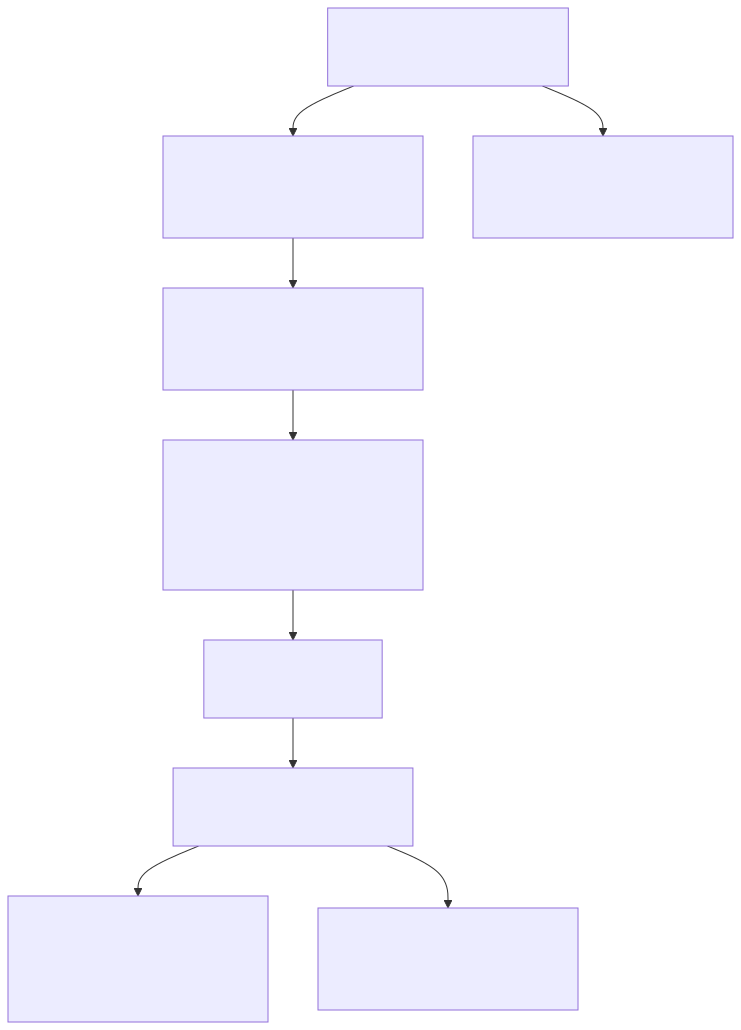
\includegraphics[keepaspectratio,width=\maxwidth,alt={Mermaid Diagram 1}]{generated/0010-automatic-path-discovery/mermaid_1.png}}

Fig. 1: Network topology for BFA inspired network probing

The probing traffic from node \texttt{A} would follow the BFA pattern of
establishing the telemetry from the immediate vicinity of \texttt{A}
using a 1-hop probing traffic:

\begin{Shaded}
\begin{Highlighting}[]
\NormalTok{A {-}\textgreater{} B {-}\textgreater{} A}
\NormalTok{A {-}\textgreater{} C {-}\textgreater{} A}
\NormalTok{A {-}\textgreater{} D {-}\textgreater{} A}
\end{Highlighting}
\end{Shaded}

Once the immediate vicinity is probed, a larger share of the probing
traffic SHOULD use the depth-first algorithm phasing the BFA into
smaller proportion.

\subparagraph{4.2.1.2 Depth-first algorithm
(DFA)}\label{4212-depth-first-algorithm-dfa}

Depth-First Search (DFS) is a graph traversal algorithm that explores as
far as possible along each branch before backtracking. It MUST start at
the current node to explore each branch of the graph deeply before
moving to another branch.

DFS is particularly useful for solving problems related to maze
exploration and pathfinding.

This algorithm SHOULD be primarily implemented in terms of the
\textbf{n-hop to self}, where \texttt{n\ \textgreater{}\ 1} and
\texttt{n\ \textless{}\ MAX\_HOPR\_SUPPORTED\_PATH\_LENGTH} (a network
parameter defined in
\href{../RFC-0004-hopr-packet-protocol/0004-hopr-packet-protocol.md}{RFC-0004}),
with each edge probed as soon as feasible, but at the same time not at
the expense of other edges in the topology. \texttt{n} SHOULD be chosen
randomly, but MUST conform with the minimum requirement for edge
traversal.

Given a network topology around the node A (Fig. 2):

\pandocbounded{\includegraphics[keepaspectratio,width=\maxwidth,alt={Mermaid Diagram 2}]{generated/0010-automatic-path-discovery/mermaid_2.png}}

Fig. 2: Network topology for DFA inspired network probing

The probing traffic from node \texttt{A} would follow the DFA pattern of
establishing the telemetry to the furthest interesting point in the
network using an \texttt{n}-hop probing traffic with \texttt{n}
generated randomly:

\begin{Shaded}
\begin{Highlighting}[]
\NormalTok{A {-}\textgreater{} B {-}\textgreater{} F {-}\textgreater{} A}
\NormalTok{A {-}\textgreater{} C {-}\textgreater{} F {-}\textgreater{} E {-}\textgreater{} A}
\NormalTok{A {-}\textgreater{} B {-}\textgreater{} D {-}\textgreater{} A}
\end{Highlighting}
\end{Shaded}

\subparagraph{4.2.1.3 BFA and DFA
interactions}\label{4213-bfa-and-dfa-interactions}

Average values calculated over the differences of various observations
can be used to establish individual per node properties. From the
previous example, given multiple averaged telemetry values over the path
it is possible to establish ensemble information about the topology.

Example: With average path latencies observed over these paths as:

\begin{Shaded}
\begin{Highlighting}[]
\NormalTok{A {-}\textgreater{} B {-}\textgreater{} A = 421ms}
\NormalTok{A {-}\textgreater{} B {-}\textgreater{} F {-}\textgreater{} A = 545ms}
\end{Highlighting}
\end{Shaded}

It is possible to establish the average latency of introducing the node
\texttt{F} into the path as
\texttt{A\ -\textgreater{}\ B\ -\textgreater{}\ F\ -\textgreater{}\ A} -
\texttt{A\ -\textgreater{}\ B\ -\textgreater{}\ A}= 545 - 421 = 124ms.

Assuming artificial mixer delays introducing additional anonymity,
repeated observations of this value averaged over longer windows would
provide an average expected latency introduced by element \texttt{F}.

\paragraph{4.2.2 Evaluation mechanism}\label{422-evaluation-mechanism}

Evaluation mechanism SHOULD have short-term memory and equally reward
and penalize probe success and failures.

\paragraph{4.2.3 Retention and slashing
mechanism}\label{423-retention-and-slashing-mechanism}

Nodes MAY implement a slashing mechanism based on failed probes to avoid
using the relay nodes in non-probing communication and avoid dropped
messages.

\paragraph{4.2.4 Throughput
considerations}\label{424-throughput-considerations}

Paths SHOULD be used by the discovery mechanism in a way that would
allow sustained throughput, i.e. the maximum achievable packet rate:

\begin{itemize}
\tightlist
\item
  Calculate load balancing over paths based on the min stake on the path
\item
  Actual throughput as measured by the real traffic
\end{itemize}

\subsubsection{4.3. Telemetry}\label{43-telemetry}

Refers to data and metadata collected by the probing mechanism about the
traversed transport path.

\paragraph{4.3.1 Next-hop telemetry}\label{431-next-hop-telemetry}

Supplemental per path telemetry (PPT) MUST be used as a source of
information for a possibly channel opening and closing strategy
responsible for reorganizing the first hop connections from the current
node.

The PPT SHOULD provide the basic evaluation of the transport channel in
the absence of an open onchain channel and MUST provide at least these
transport channel observations using 0-hop as specified in the HOPR
protocol
\href{../RFC-0004-hopr-packet-protocol/0004-hopr-packet-protocol.md}{RFC-0004}:

\begin{enumerate}
\def\labelenumi{\arabic{enumi}.}
\tightlist
\item
  latency

  \begin{itemize}
  \tightlist
  \item
    duration between a send-message and a corresponding acknowledgement
  \end{itemize}
\item
  packet drop

  \begin{itemize}
  \tightlist
  \item
    track ratio of missing/all expected acknowledgements for each
    message on the channel
  \end{itemize}
\end{enumerate}

The PPT MAY be utilized as an information source by other mechanisms,
e.g. the channel manipulation strategy optimizing the outgoing network
topology.

\paragraph{4.3.2 Non-probing telemetry}\label{432-non-probing-telemetry}

The non-probing telemetry MAY track the next-hop telemetry targets with
the goal of adding more relevant channel information for the nearest
0-hop.

Each outgoing message should be tracked for the same set of telemetry as
the PPT on the per message basis.

\paragraph{4.3.3 Probing telemetry}\label{433-probing-telemetry}

Telemetry data pertains to the content of the probing message sent over
the network. All multi-byte integer fields MUST be transmitted in
network byte order (big endian).

The content of the probing message:

\begin{itemize}
\tightlist
\item
  Iterating counter to verify the mixing property over a path

  \begin{itemize}
  \tightlist
  \item
    an iterated \texttt{uint64} equivalent value
  \end{itemize}
\item
  Path identification for attribution

  \begin{itemize}
  \tightlist
  \item
    a unique value identifying a single specific path in the graph using
    a \texttt{uint64} equivalent value
  \end{itemize}
\item
  Timestamp of packet creation for channel latency observations

  \begin{itemize}
  \tightlist
  \item
    formatted as an 8-byte (64-bit) \texttt{UNIX\ time\ in\ nanoseconds}
  \end{itemize}
\end{itemize}

\begin{Shaded}
\begin{Highlighting}[]
\NormalTok{+{-}{-}{-}{-}{-}{-}{-}{-}{-}{-}{-}{-}{-}+{-}{-}{-}{-}{-}{-}{-}{-}{-}{-}{-}{-}+{-}{-}{-}{-}{-}{-}{-}{-}{-}{-}{-}{-}+}
\NormalTok{|   Counter   |   PathId   |  Timestamp |}
\NormalTok{|     8B      |     8B     |     8B     |}
\NormalTok{+{-}{-}{-}{-}{-}{-}{-}{-}{-}{-}{-}{-}{-}+{-}{-}{-}{-}{-}{-}{-}{-}{-}{-}{-}{-}+{-}{-}{-}{-}{-}{-}{-}{-}{-}{-}{-}{-}+}
\end{Highlighting}
\end{Shaded}

The total packet size is 24 bytes.

\subsubsection{4.4 Component placement}\label{44-component-placement}

The network probing functionality, with the exception of the PPT
mechanism, MUST be implemented using HOPR loopback communication.

Implementation requirements:

\begin{itemize}
\tightlist
\item
  The concept of channel graph quality based on network observations
  SHALL be removed

  \begin{itemize}
  \tightlist
  \item
    Only the onchain channel information SHALL be retained
  \end{itemize}
\item
  Implementations MUST provide processes to:

  \begin{itemize}
  \tightlist
  \item
    Generate a low-rate continuous stream of network path probes
  \item
    Generate session-specific paths for session path selection
    obfuscation
    \href{../RFC-0008-session-protocol/0008-session-protocol.md}{RFC-0008}
  \end{itemize}
\item
  A new path graph system SHALL be derived from these processes
\item
  Paths SHALL be cached for a configurable minimum time window
\item
  Session metrics SHALL incorporate:

  \begin{itemize}
  \tightlist
  \item
    Session-level performance metrics
  \item
    Session-specific path probing data
  \item
    Session-derived cover traffic for exploratory network traversal
  \end{itemize}
\end{itemize}

\subsection{5. Design considerations}\label{5-design-considerations}

Each sender SHOULD:

\begin{itemize}
\tightlist
\item
  Be able to identify a sufficiently large number of network nodes to
  ensure privacy through path pool diversity
\item
  Be capable of detecting unstable, malicious, or adversarial nodes
\item
  Be able to establish basic propagation metrics for Quality of Service
  (QoS) estimation
\end{itemize}

Given the capabilities described above, the message sender SHOULD be
able to construct a functional representation of the network topology,
state, and constraints, enabling optimal selection and exclusion of
message propagation paths.

The multihop probing traffic and measurement packets MUST be
indistinguishable from ordinary traffic to ensure accurate recording of
network node propagation characteristics. Due to the dynamic nature of
decentralized peer-to-peer networks, the message sender SHOULD employ
adaptive mechanisms for establishing and maintaining topological
awareness.

For both unidirectional and bidirectional communication to adapt to
changing network conditions, the sender MUST actively probe the network
in a continuous manner.

The measurement traffic itself SHOULD adhere to economic feasibility
constraints, i.e., it SHOULD be proportional to actual message traffic
and MAY be incorporated as part of the Cover Traffic (CT)
\href{../RFC-0008-session-protocol/0008-session-protocol.md}{RFC-0008}.

Any measurements obtained from the probing traffic SHOULD be
node-specific and MUST NOT be subject to data or topology exchange with
other nodes.

The collected telemetry for measured paths:

\begin{itemize}
\tightlist
\item
  MUST contain path passability data

  \begin{itemize}
  \tightlist
  \item
    Path traversability by single or multiple messages
  \end{itemize}
\item
  MAY include additional information

  \begin{itemize}
  \tightlist
  \item
    Telemetry transferred as message content
  \end{itemize}
\end{itemize}

By designing probing traffic to be indistinguishable from actual message
propagation in the mixnet, direct verification of immediate peer
properties becomes infeasible. For this purpose, a separate mechanism
not described in this document SHOULD exist.

The nearest one-hop probing mechanism MAY NOT comply with the anonymity
requirement, since it:

\begin{enumerate}
\def\labelenumi{\arabic{enumi}.}
\tightlist
\item
  mimics the 0-hop session
  \href{../RFC-0008-session-protocol/0008-session-protocol.md}{RFC-0008}
  which does not fully benefit from relaying mechanisms
\item
  could be used as a first layer for relayers to discover viable
  candidates for future channel openings
\end{enumerate}

The network probing mechanism SHALL utilize graph-based algorithms to
efficiently discover and maintain network topology information.

\subsection{6. Compatibility}\label{6-compatibility}

This feature affects only a single node in the network and MAY be
modified without impacting overall network operation.

The network probing mechanism MAY be compatible with the loopback
session mechanism

\subsection{7. Security Considerations}\label{7-security-considerations}

The probing traffic consumes both physical resources and value at
various levels of the HOPR protocol stack.

Security considerations related to resource utilization include:

\begin{enumerate}
\def\labelenumi{\arabic{enumi}.}
\tightlist
\item
  In highly volatile networks, adversarial behavior may cause excessive
  resource expenditure, potentially enabling resource depletion attacks.
\item
  The PPT mechanism MAY serve as an attack vector for Denial of Service
  (DoS) attempts.
\item
  Nodes MAY implement any security risk mitigation strategy
\end{enumerate}

\subsection{8. Drawbacks}\label{8-drawbacks}

The network probing mechanism has several inherent limitations:

\begin{enumerate}
\def\labelenumi{\arabic{enumi}.}
\tightlist
\item
  Probing activity consumes resources; implementations MUST carefully
  balance probing and data transmission activities to maintain
  reasonable resource utilization ratios.
\item
  Complete real-time probing of large networks is computationally
  prohibitive; algorithms SHOULD operate within bounded subnetworks
  where they can provide reasonable network visibility guarantees.
\item
  Prior knowledge of target nodes is advantageous to minimize
  initialization time before establishing a sufficient network view for
  informed path selection.
\end{enumerate}

\subsection{9. Alternatives}\label{9-alternatives}

No alternative mechanisms exist that simultaneously preserve anonymity,
maintain trustless properties, and consolidate probing control under the
communication source.

\subsection{10. Unresolved Questions}\label{10-unresolved-questions}

None

\subsection{11. Future Work}\label{11-future-work}

Future development SHOULD focus on:

\begin{enumerate}
\def\labelenumi{\arabic{enumi}.}
\tightlist
\item
  Improving the ability to collect additional network metrics primarily
  by extending the data payload transmitted along the loopback path
\item
  Developing new path generating strategies allowing statistical
  inference of information from the path section overlaps
\item
  Improve metric evaluation mechanism
\item
  Add proper slashing mechanism with equation based logic
\end{enumerate}

\subsection{12. References}\label{12-references}

\begin{itemize}
\tightlist
\item
  \href{../RFC-0002-mixnet-keywords/0002-mixnet-keywords.md}{RFC-0002}
  -- Mixnet terminology
\item
  \href{../RFC-0004-hopr-packet-protocol/0004-hopr-packet-protocol.md}{RFC-0004}
  -- HOPR packet protocol
\item
  \href{../RFC-0005-proof-of-relay/0005-proof-of-relay.md}{RFC-0005} --
  Proof of Relay
\item
  \href{../RFC-0007-economic-reward-system/0007-economic-reward-system.md}{RFC-0007}
  -- Economic Reward System
\item
  \href{../RFC-0008-session-protocol/0008-session-protocol.md}{RFC-0008}
  - Session Data Protocol
\end{itemize}
